%! Mode:: "TeX:UTF-8"
%! TEX program = xelatex
\PassOptionsToPackage{quiet}{xeCJK}
\documentclass[withoutpreface,bwprint]{cumcmthesis}
\usepackage{etoolbox}
\BeforeBeginEnvironment{tabular}{\zihao{-5}}
\usepackage[numbers,sort&compress]{natbib}  % 文献管理宏包
\usepackage[framemethod=TikZ]{mdframed}  % 框架宏包
\usepackage{url}  % 网页链接宏包
\usepackage{subcaption}  % 子图宏包
\newcolumntype{C}{>{\centering\arraybackslash}X}
\newcolumntype{R}{>{\raggedleft\arraybackslash}X}
\newcolumntype{L}{>{\raggedright\arraybackslash}X}


%%%%%%%%%%%%%%%%%%%%%%%%%%%%%%%%%%%%%%%%%%%%%%%%%%%%%%%%%%%%%
% 论文标题
\title{基于深度展开模拟分叉算法求解多收发信号检测问题}


%%%%%%%%%%%%%%%%%%%%%%%%%%%%%%%%%%%%%%%%%%%%%%%%%%%%%%%%%%%%%
%% 正文
\begin{document}

\maketitle
\begin{abstract}
量子退火启发算法 (QAIA) 近年来被用于求解通信领域中的多收发系统 (MIMO) 信号检测问题,本赛题要求选手设计一个基于 QAIA 原理的 MIMO 检测算法。
本文在复现文献 \cite{Takabe2023} 所提出的 DU-LM-SB 方法基础上继续加以改进,提出并探索了 pReg-LM-SB 系列方法以试图进一步降低比特误差率或提高解码速度。
若仅考虑比特误差,我们提交的最好方案比特误码率可低至 0.18597,相比基线降低 54.77\%;
若兼顾运行时间,则我们改进出的方案在线评测分数可达 105.2462 分。

\keywords{量子退火启发算法 \quad QAIA \quad 模拟分叉 \quad 深度展开 \quad MIMO检测}
\end{abstract}


%%%%%%%%%%%%%%%%%%%%%%%%%%%%%%%%%%%%%%%%%%%%%%%%%%%%%%%%%%%%%
% 目录
% \tableofcontents
% \newpage


%%%%%%%%%%%%%%%%%%%%%%%%%%%%%%%%%%%%%%%%%%%%%%%%%%%%%%%%%%%%%
\section{问题背景}

量子退火启发算法 (QAIA) 是一类受到量子退火或绝热演化等动力学过程启发而提出的经典算法,可用于求解组合优化等问题,
具体包括模拟相干伊辛机 (SimCIM)、含噪平均场退火 (NMFA)、模拟分叉 (SB) 等诸多算法。
多收发系统 (MIMO) 是信号通信领域中用于在共享信道中大规模数据传输的技术,
MIMO 信号检测问题即如何从多根天线的接收数据中独立恢复出多个发射源信息的问题。
近年来有不少工作尝试使用量子退火或相关的启发算法来解决 MIMO 检测问题,是一个有潜力的新兴研究方向。


%%%%%%%%%%%%%%%%%%%%%%%%%%%%%%%%%%%%%%%%%%%%%%%%%%%%%%%%%%%%%
\section{问题分析}

本赛题要求选手在建模和算法方面进行探索,设计一个基于 QAIA 原理的 MIMO 检测算法,同时追求低误码率和高计算性能。
MIMO通信原理可用图 \ref{fig:mimo} 和 公式 \ref{eq:mimo} 来简单描述,即发送比特数据 $ \mathrm{bits} $ 调制后的信号 $ \mathrm{x} $ 经过多路信道 $ \mathrm{H} $ 的传输,受到信道噪声 $ \mathrm{n} $ 干扰后,接收方读出信号数据为 $ \mathrm{y} $。
MIMO检测问题即在给定接受信号 $ \mathrm{y} $ 和信道矩阵 $ \mathrm{H} $ 的基础上恢复发送比特数据 $ \mathrm{bits} $。

\begin{figure}[h!]
	\centering
	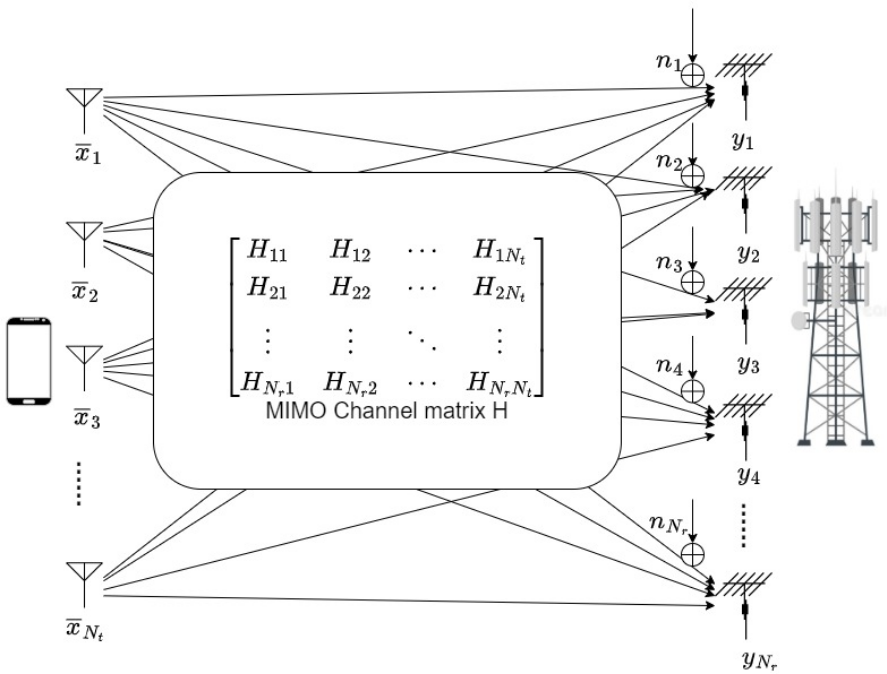
\includegraphics[scale=0.37]{figures/mimo.png}
	\caption{MIMO系统示意图}
	\label{fig:mimo}
\end{figure}

\begin{equation}
\begin{split}
\mathrm{x} &= \mathrm{modem}(\mathrm{bits}) \\
\mathrm{y} &= \mathrm{x} \mathrm{H} + \mathrm{n} \\
\end{split}
\label{eq:mimo}
\end{equation}

Singh 等人 \cite{Singh2021} 将 MIMO 问题映射为组合优化问题,从首次实现了将 SimCIM 算法应用于 MIMO 检测问题求解。
同年 Goto 提出的模拟分叉算法 (SB, Simulated Bifurcation) \cite{Goto2021} 受启发于复杂系统中的分叉现象,可用于在经典计算机上高效地解决组合优化问题。
基于此,Takabe \cite{Takabe2023} 用 SB 替代 SimCIM 进行 MIMO 检测,获得了更好的结果,具体做法流程如下:
首先按公式 \ref{eq:to-ising-0} 将复信道矩阵 $ \mathrm{H} $ 平坦化为实矩阵,进一步按公式 \ref{eq:to-ising-1} 构造出 Ising 模型中的耦合系数矩阵 $ \mathrm{J} $ 与外场向量 $ \mathrm{h} $,
随后运行 SB 算法使用辛几何欧拉方法 (symplectic Euler method) 迭代求解关于系统哈密顿量 $ H_{SB} $ 的偏微分方程组 \ref{eq:sb} 得到自旋向量 $ x $,
最后从自旋形式 $ \{-1,1\} $ 转换为比特形式 $ \{0,1\} $ 得到恢复后的数据比特。

\begin{equation}
\tilde{\mathrm H} = \begin{bmatrix}
   Re(\mathrm H) & -Im(\mathrm H) \\
   Im(\mathrm H) &  Re(\mathrm H) \\ 
\end{bmatrix},
\tilde{\mathrm y} = \begin{bmatrix}
   Re(\mathrm y)  \\
   Im(\mathrm y) \\ 
\end{bmatrix} \\
\label{eq:to-ising-0}
\end{equation}

\begin{equation}
\begin{split}
\mathrm T &= \begin{bmatrix}
   2^{r_b-1} \mathcal I_N & 2^{r_b-2} \mathcal I_N & \dots & \mathcal I_N
\end{bmatrix} \\
z &= \tilde{\mathrm y} - \tilde{\mathrm H} \mathrm T \bar{1}_{N*r_b} + (\sqrt M - 1) \tilde{\mathrm H} \bar{1}_N \\
J &= -zeroDiag(\mathrm T^T \tilde{\mathrm H}^T \tilde{\mathrm H} \mathrm T) \\
h &= 2 * z^T \tilde{\mathrm H} \mathrm T \\
\end{split}
\label{eq:to-ising-1}
\end{equation}

\begin{equation}
\begin{split}
\frac{\partial H_{SB}}{\partial y_i} &= a_0 y_i \\
\frac{\partial H_{SB}}{\partial x_i} &= -[a_0 - a(t)] x_i + c_0 (\sum\limits_{j=1}^N J_{i,j} x_j + h_j) \\
\end{split}
\label{eq:sb}
\end{equation}


%%%%%%%%%%%%%%%%%%%%%%%%%%%%%%%%%%%%%%%%%%%%%%%%%%%%%%%%%%%%%
\section{解决方案}

我们的解决方案主要包含三部分:复现论文 \cite{Takabe2023} 中的三种方法、提出我们的 pReg-LM-SB 系列方法、运行效率优化。

\subsection{DU-LM-SB方法}

文献 \cite{Takabe2023} 中引述了三种方法,其关系为递进式的改进:
首先是基线方法 ML-SB,即使用上一节中提到的信道矩阵转Ising模型公式 \ref{eq:to-ising-1} 搭配原始的 SB 算法;
然后是引入正则项的改进方法 LM-SB,即按照公式 \ref{eq:to-ising-du} 向 $ \mathrm{J} $ 和 $ \mathrm{h} $ 中引入了一个 LMMSE-like 的矩阵作为正则项,以尽量避免 SB 算法陷入局部最优解,降低了误差底线;
最后是引入深度展开技术 (DU, deep unfold) 的改进方法 DU-LM-SB,通过梯度下降反向传播来实现 SB 算法中一些超参数的自动调参,并极大降低算法所需要的迭代步数,基本思想类似于 QAOA 算法用有限离散步来模拟连续的退火过程。

\begin{equation}
\begin{split}
\mathrm U_\lambda &= (\mathrm H \mathrm H^T + \lambda I)^{-1} \\
J &= -zeroDiag(\mathrm T^T \tilde{\mathrm H}^T \mathrm U_\lambda \tilde{\mathrm H} \mathrm T) \\
h &= 2 * z^T \mathrm U_\lambda \tilde{\mathrm H} \mathrm T \\
\end{split}
\label{eq:to-ising-du}
\end{equation}

在实现 LM-SB 方法时,其中的 $ \lambda $ 是一个需要手动调节的超参数,原论文设置为 1。
但我们发现在比赛给定的数据集上,无论怎么调节这个常数,算法性能都不好。
于是我们进一步将 $ \mathrm U_\lambda $ 的定义改造为公式 \label{eq:U-lmbd},并发现此时取 $ \lambda = 25 $ 是一个不错的选择。
在实现 DU-LM-SB 方法时,有一个难点是将 SB 算法和 ber 损失函数改造成可微函数,以实现端到端梯度传递,
具体实现比较繁琐而富有技巧,可参考附录和我们提交的代码。

\begin{equation}
\mathrm U_\lambda = (\mathrm H \mathrm H^T + \lambda I)^{-1} / \lambda \\
\label{eq:U-lmbd}
\end{equation}

\subsection{pReg-LM-SB方法}

注意到 LM-SB 方法中引入了一个瓶颈矩阵 $ \mathrm U_\lambda $,它既含有样本相关的部分即 $ \mathrm H \mathrm H^T $,也含有样本无关的部分即 $ ([\cdot] + \lambda I)^{-1} $ 结构。
且在进一步的 DU-LM-SB 方法中,可学习参数只有一个参量 $ \lambda $,于是我们想到可以进一步提高这个正则项的可学习程度,从而引出了 pReg-LM-SB 系列方法,即在 DU-LM-SB 方法的基础上进一步探索:

\begin{itemize}
\item pReg-LM-SB:将 $  \lambda I $ 部分替换为一个可学习的对称矩阵
\item ppReg-LM-SB:将整个 $ \mathrm U_\lambda $ 替换为一个可学习的对称矩阵
\end{itemize}

\subsection{运行效率优化}

按赛题评分公式,我们发现在比特误差率超过基线的条件下,选手所提交的算法运行效率是一个极大的加分因素,因此我们对程序进行了多方面的性能优化:

\begin{itemize}
\item 借助深度展开技术,极大降低 SB 算法所需迭代轮数 (n\_iter=6)
\item 在 SB 算法中使用 batch\_size=1,即仅使用一组自旋向量
\item 使用稠密矩阵表示,而非稀疏矩阵运算库 scipy.sparse,因为信道矩阵 $ \mathrm H $ 并不稀疏
\item 借助矩阵乘法结合律,精心调整矩阵运算的顺序以最小化计算量
\item 缓存频繁访问的中间结果和辅助数据
\item 使用\textbf{近似运算}求矩阵的逆
\end{itemize}

\begin{equation}
\mathrm A^{-1} \approx \sum\limits_{i=0}^n (\mathrm I - \mathrm A)^i
\label{eq:neumann}
\end{equation}

这里只展开介绍最后一项,即我们发现引入的正则项部分 $ \mathrm U_\lambda $ 的矩阵求逆操作成了最后唯一难以优化的性能瓶颈,必须想办法做近似计算。
注意到这个正则项在数值上其实非常接近于于一个单位矩阵,可以截断如公式 \ref{eq:neumann} 所示的诺伊曼级数 (Neumann series) 对其进行近似展开。
但这个展开仍需求矩阵的高阶次幂,虽然在精确计算的意义上可以使用华罗庚公式展开,但是我们发现需要截断到大约前 24 项才能取得较好的近似效果,还是比较慢。
在这里我们偶然地 (wtf?!) 发现了一个近似方法,只需要 5 步迭代就能取得较好的近似结果,具体做法可参考附录或提交的代码。


%%%%%%%%%%%%%%%%%%%%%%%%%%%%%%%%%%%%%%%%%%%%%%%%%%%%%%%%%%%%%
\section{结果}

我们首先给出 Sionna库 \cite{sionna2022} 所提供的各传统方法在比赛给定数据集上的性能表现,此处仅考虑比特错误率 (BER, bit errir rate) 指标。
如表 \ref{tbl:result-c} 所示,其中 linear-zf-maxlog 即比赛所指定的基线方法 Zero-Forcing,而 ep-iter=10 即 10 步迭代的 Expectation Propagation 方法 \cite{Wang2020} 有最低的比特错误率 0.16872。
其中被删除线划去的 mmse-iter=8 虽然看似有更低的比特错误率 0.15738,实则加入了真实目标值作为正则项来进行优化,故这个最低数字标定了比赛所提供的数据集在一般方法上所能达到的最低理论误差下限。

其次我们给出 Mindquantum 库 \cite{mindquantum2021} 所提供的各类基于QAIA的算法在比赛给定数据集上的性能表现。
如表 \ref{tbl:result-q} 所示,可见 SB 系列算法最优情况 (BER=0.21584) 确实超越了此研究方向根论文所使用的 SimCIM (BER=0.23271)。
进一步复现验证文献 \cite{Takabe2023} 可得到结果 LM-bSB-λ=25 (BER=0.18591) 和 DU-LM-SB-T=30 (BER=0.19497),均优于朴素 SB。
但 DU-LM-SB 相对于 LM-SB 而言,并未展现出论文中所报道的显著优势。

\begin{minipage}{\textwidth}
\begin{minipage}[t]{0.45\textwidth}
	\centering
	\makeatletter\def\@captype{table}\makeatother
	\caption{基于传统方法的对比算法\label{tbl:result-c}}
	\begin{tabular}{cc} 
		\textbf{算法} 			& \textbf{比特错误率↓} \\
		\hline
		linear-zf-maxlog		& \underline{0.41121} \\
		linear-zf-app			& 0.40605 \\
		linear-mf-maxlog		& 0.34104 \\
		linear-mf-app		& 0.33401 \\
		linear-lmmse-maxlog	& 0.20779 \\
		linear-lmmse-app		& 0.20721 \\
		kbest-k=64			& 0.26206 \\
		ep-iter=10			& \textbf{0.16872} \\
		mmse-iter=8			& \sout{0.15738} \\
	\end{tabular}
\end{minipage}
\begin{minipage}[t]{0.45\textwidth}
	\centering
	\makeatletter\def\@captype{table}\makeatother
	\caption{基于量子退火启发的对比算法\label{tbl:result-q}}
	\begin{tabular}{cc}        
		\textbf{算法} 						& \textbf{比特错误率↓} \\
		\hline
		NMFA   							& 0.38561 \\
		SimCIM \cite{Singh2021} 			& 0.23271 \\
		CAC    							& 0.31591 \\
		CFC    							& 0.23801 \\
		SFC    							& 0.23796 \\
		ASB    							& 0.34054 \\
		DSB   							& 0.28741 \\
		BSB \cite{Goto2021} 				& 0.21584 \\
		LQA   							& 0.20627 \\
		LM-bSB-λ=25 \cite{Takabe2023} 	& 0.18591 \\
		DU-LM-SB-T=30 \cite{Takabe2023}	& 0.19497 \\
	\end{tabular}
\end{minipage}
\end{minipage}

最后我们给出经过我们极致优化后的 LM-SB 和 DU-LM-SB 方法的配置,以及我们提出的 pReg-LM-SB 方法的实验结果。
如表 \ref{tbl:result} 所示,当 SB 算法的迭代次数 n\_iter=100,自旋向量的候选数量 B=10 时,LM-SB 方法能取得最低的误码率 BER=0.18656。
进一步降低这两项参数会有效降低运行时间而提高分数,但也会导致误码率的急剧上升,直到 n\_iter=10,B=1 时,误码率已接近基线的一半 BER=0.21345。
此时我们只能引入 DU 技术来保证误码率不降低太多的条件下,进一步降低迭代次数到 n\_iter=6。
此时发现矩阵求逆称为主要的性能瓶颈,采用近似算法之后可将运行时间缩短至一半,虽然误码率有一定的提升,但总分加权而言还是有非常可观的提升,取得了我们的有效最高分 105.2462 分。
对于另一方面针对 pReg-LM-SB 方法的探索,可见它与未经近似矩阵逆优化的 DU-LM-SB 相比性能完全持平;而完全不需要求矩阵逆的 ppReg-LM-SB 则更是同时在误码率和速度上都出类拔萃。
但需要注意的是,该方法是过拟合训练集的结果,它与上文 mmse-iter=8 一样,在一定程度上反映了任何方法在比赛给定数据集上可能达到的最高理论分数上限。
图 \ref{fig:result-cmp} 给出了以朴素SB算法作为基线,与我们最好的方法配置作对比的各样本 BER 值 (分别按降序排列),可以看到基本轮廓保持了一致,但均值有明显的降低。

\begin{table}[h!]
	\centering
	\caption{我们优化后的算法实验结果}
	\begin{tabular}{llllll}
		\textbf{方法} & \textbf{比特错误率↓} & \textbf{运行时间↓} & \textbf{本地估分↑} & \textbf{提交评分↑} & \textbf{算法参数配置} \\
		\hline
		LM-SB & \textbf{0.18656} &  36.39 &  5.2332 &  4.9567 & B=10, n\_iter=100 \\
		LM-SB & 0.21345 & 2.72 & 67.5861 & 92.4872 & B=1, n\_iter=10 \\
		DU-LM-SB & 0.19932 & 2.73 & 68.5260 & 89.3023 & B=1, n\_iter=10 \\
		DU-LM-SB & 0.20696 & 2.65 & 70.0280 & - & B=1, n\_iter=6 \\
		DU-LM-SB & 0.21805 & 1.37 & 133.5814 & \textbf{105.2462} & B=1, n\_iter=6, approx \\
		pReg-LM-SB & 0.19940 & 2.77 & 67.6817 & 92.9875 & B=1, n\_iter=10 \\
		ppReg-LM-SB & 0.15490 & 1.26 & 156.9497 & \sout{137.3652} & B=1, n\_iter=10, overfit \\
	\end{tabular}
	\label{tbl:result}
\end{table}

\begin{figure}
	\centering
	\subcaptionbox{SB算法基线}
	{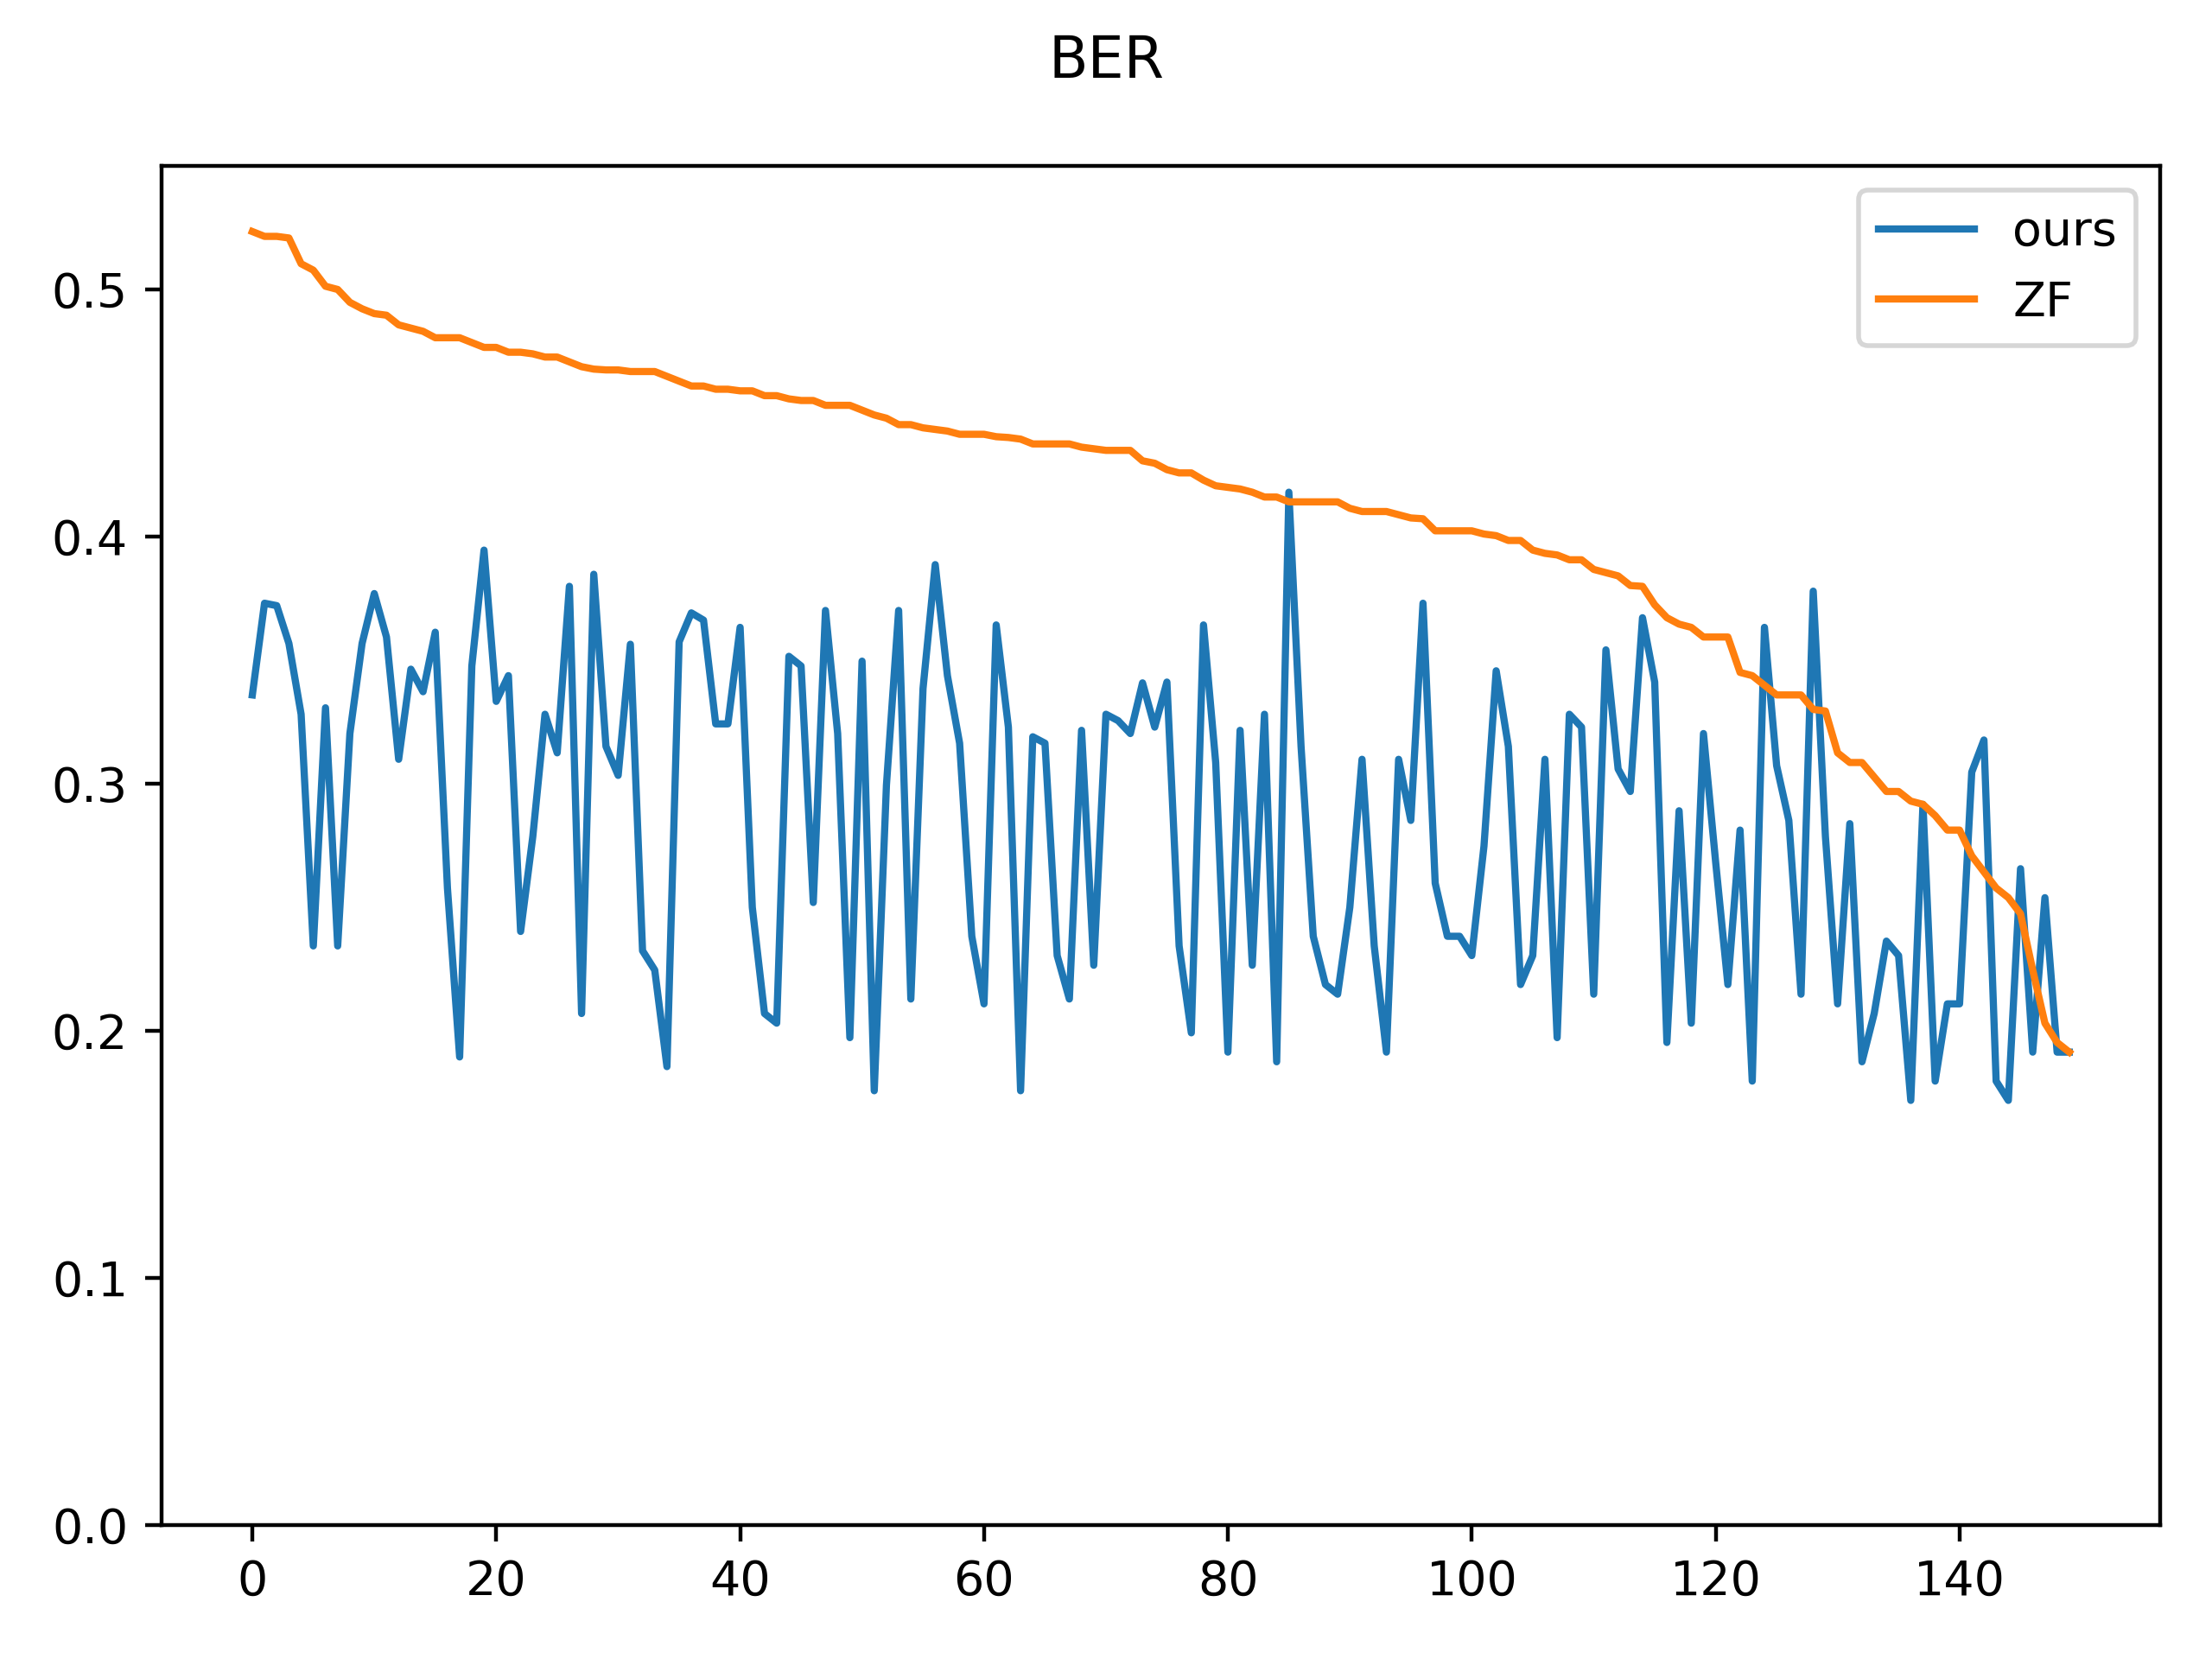
\includegraphics[width=0.48\textwidth]{figures/solut-baseline.png}}
	\subcaptionbox{我们的最优算法设置}
	{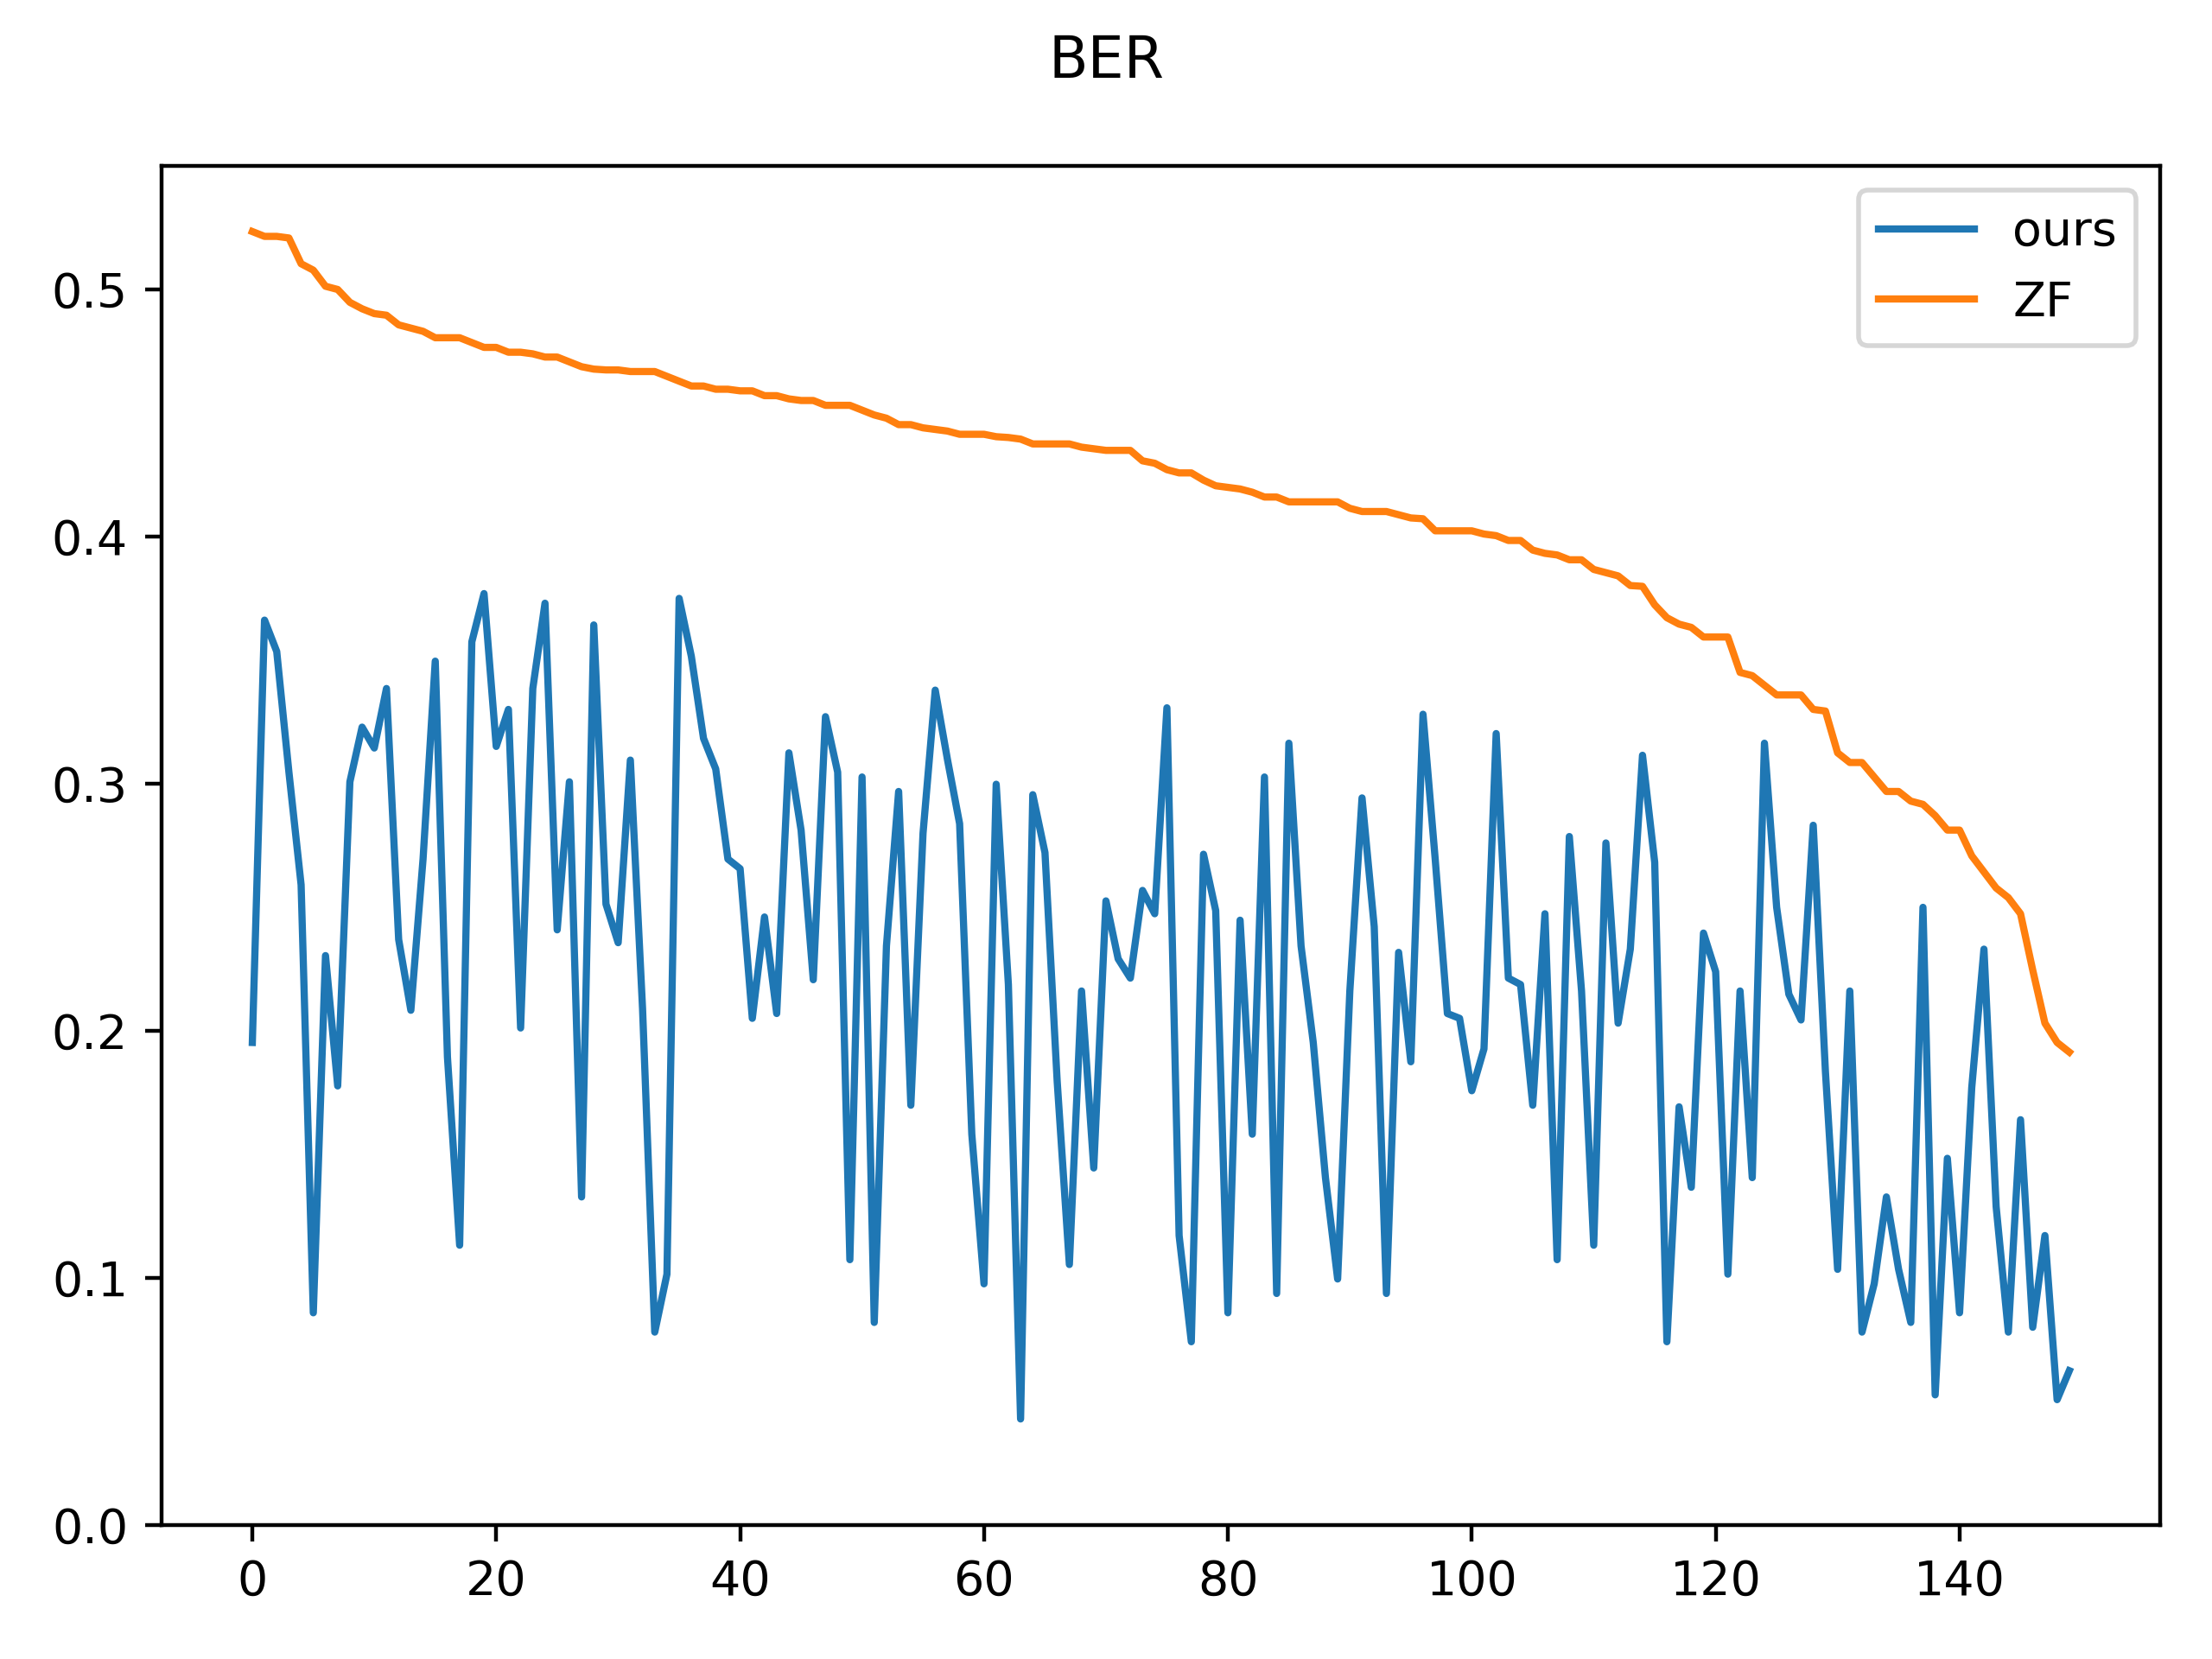
\includegraphics[width=0.48\textwidth]{figures/solut-ours.png}}
	\caption{SB基线与我们的方法BER对比}
	\label{fig:result-cmp}
\end{figure}


%%%%%%%%%%%%%%%%%%%%%%%%%%%%%%%%%%%%%%%%%%%%%%%%%%%%%%%%%%%%%
\section{总结及展望}

本文探索了基于 QAIA 算法求解 MIMO 检测问题,复现了 DU-LM-SB 系列的论文并加以调整改进,探索了自主提出的 pReg-LM-SB 方法。
我们为程序运行效率做了精心的优化,并提出了基于截断诺伊曼级数来近似矩阵求逆。
最终我们优化出来的方法最高可达到 105.2462 分,与估计出来的可能最优分数上限 137.3652 仍有约 23.38\% 的差距,仍待继续探索。
只是无论面对任何方法,当我们对信道噪声难以估计的时候,MIMO检测问题都仍会是困难的;未来的进路可能由此铺开。


%%%%%%%%%%%%%%%%%%%%%%%%%%%%%%%%%%%%%%%%%%%%%%%%%%%%%%%%%%%%%
%% 参考文献
\newpage

\nocite{*}
\bibliographystyle{gbt7714-numerical}  % 引用格式
\bibliography{ref.bib}  % bib源


%%%%%%%%%%%%%%%%%%%%%%%%%%%%%%%%%%%%%%%%%%%%%%%%%%%%%%%%%%%%%
%% 附录
\newpage
\begin{appendices}

\section{主要代码}

MIMO 问题转 Ising 模型:

\lstinputlisting[language=python]{code/to_ising.py}

\newpage
可微分的BER损失函数:

\lstinputlisting[language=python]{code/diff_ber_loss.py}

\newpage
可微分的SB算法过程:

\lstinputlisting[language=python]{code/diff_sb.py}

\end{appendices}
\end{document}